\begin{XeClass}{AbstractFileSystem}
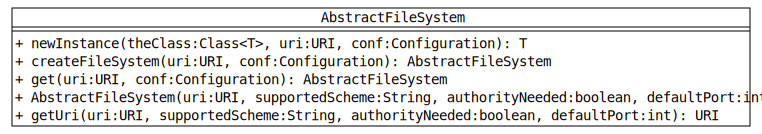
\includegraphics[width=\textwidth]{cdig/AbstractFileSystem.png}
     
 AbstractFileSystem(下简称AFS)是提供给Hadoop FS体系下的具体文件系统实现者的接口.
 AFS以抽象类的形式向Hadoop FS中的具体文件系统的实现者提供接口.
 Hadoop FS的架构与Unix下VFS类似, 应用不直接访问AFS实例,
 而是通过\emph{FileContext}实例来访问文件系统中的文件.
 传递给AFS的路径(pathnames)可以是符合具体文件系统规定的、完全限定的URI,
 也可以是以给定文件系统的根目录为'/'目录的, 以‘/’分隔的路径(同Unix体系).
 
 由于AbstractFileSystem本身是提供给文件系统实现者的接口,
 且Hadoop FS中对文件的访问全部由\emph{FileContext}控制, 所以,
 这个类里没有public方法, 而是提供了三类protected方法:
 
 AFS实例由工厂方法\emph{AbstractFileSystem.get(URI,Configuration)}创建.
 AFS中封装了一批通用操作的抽象方法, 这些方法由具体文件系统的实现者实现.

    \begin{XeMethod}{}{T}{newInstance}
         
 反射机制实现的初始化, URI和Configuration会被传递给实际的构造方法

    \end{XeMethod}

    \begin{XeMethod}{\XePrivate}{AbstractFileSystem}{createFileSystem}
         
 通URI和Configuration创建AFS实例,
 该方法被直接用于工厂方法\emph{AbstractFileSystem.get(URI,Configuration)}
 not found

    \end{XeMethod}

    \begin{XeMethod}{}{AbstractFileSystem}{get}
         
 创建AbstractFileSystem实例的主要工厂方法, 通过URI的体系(scheme)和权限获取文件系统.
 URI中描述的体系确定配置中一个名为
 \emph{fs.AbstractFileSystem.scheme.impl}
 的属性, 这个属性的值就是该scheme对应的AbstractFileSystem类的具体实现.
 完整的URI和配置信息会被传递给AbstractFileSystem的工厂方法, 即\emph{AbstractFileSystem.createFileSystem(URI,Configuration)}
 \emph{uri} is not supported.

    \end{XeMethod}

    \begin{XeMethod}{\XeProtected}{AbstractFileSystem}{AbstractFileSystem}
         
 子类需用的构造方法, 该方法配置实例的URI和统计信息.
 then the URI must have null authority.

    \end{XeMethod}

    \begin{XeMethod}{\XePrivate}{URI}{getUri}
         
 由给定的URI中截取文件系统根目录的URI.
 false authority must be null.

    \end{XeMethod}

\end{XeClass}
